
%----------------------------------------------------------------------------------------
%	Settings and packages
%----------------------------------------------------------------------------------------

\documentclass[10pt]{article}

\usepackage{colortbl}
\usepackage{multirow}
\usepackage[table]{xcolor}
\usepackage{ctable}
\usepackage{float}
\usepackage[landscape,margin=0.25in,legalpaper]{geometry}

\newcommand{\mcn}[2]{\multicolumn{#1}{l}{#2}}	
\newcommand{\mccn}[2]{\multicolumn{#1}{c}{#2}}
\newcommand{\mcl}[1]{\multicolumn{2}{l}{#1}}
\newcommand{\mclg}[1]{\multicolumn{2}{l}{\gr #1}}
\newcommand{\mcc}[1]{\multicolumn{2}{c}{#1}}
\newcommand{\mccg}[1]{\multicolumn{2}{c}{\gr #1}}
\newcommand{\mr}[1]{\multirow{-2}{*}{#1}}
\definecolor{Gray}{gray}{0.90}
\newcommand{\gr}{\cellcolor{Gray}}

\newcommand{\thickline}{\specialrule{.1em}{.05em}{.05em}}

\setlength\parindent{0pt}

% column colours
\newcolumntype{g}{>{\columncolor{Gray}}l}
\newcolumntype{w}{>{\columncolor{white}}l}

%----------------------------------------------------------------------------------------
%	Create new commands
%----------------------------------------------------------------------------------------

% Commands are in LatexCommands.tex. New commands for this file only can be written here.
%\input{/Applications/TeX/Latex_ancillary/LatexCommands.tex}


%----------------------------------------------------------------------------------------
%	Table
%----------------------------------------------------------------------------------------

\begin{document}

\thispagestyle{empty}
{\bf 2015 Deepwell Cup}
\begin{table}[h!]
    \centering
    \begin{tabular}{l g g w w g g w w g g w w g g w w g g w w g g}
        \rowcolor{black}\mcn{23}{\color{white}\bf Round 4: Stanley Cup Finals} \\
        \rowcolor{white}\\
        &  \mccg{Alita D}&  \mcc{Andre D}&  \mccg{Anthony C}&  \mcc{Charmaine L}&  \mccg{David D}&  \mcc{Harry L}&  \mccg{Kollin H}&  \mcc{Kyle L}&  \mccg{Mark D}&  \mcc{Michael D}&  \mccg{Thomas L} \\\thickline
          Tampa Bay Lightning&&&&&&&&&&&&&&&&&&&&&&\\
          Chicago Blackhawks & \mr{TBL} & \mr{7} & \mr{TBL} & \mr{7} & \mr{CHI} & \mr{6} & \mr{CHI} & \mr{6} & \mr{CHI} & \mr{7} & \mr{TBL} & \mr{7} & \mr{CHI} & \mr{5} & \mr{TBL} & \mr{6} & \mr{TBL} & \mr{6} & \mr{CHI} & \mr{6} & \mr{TBL} & \mr{7}\\\hline
          \rowcolor{white}\\
        \rowcolor{black} \mcn{23}{\color{white}\bf Conference Champions} \\
          Eastern & \mclg{WSH} & \mcl{NYR} & \mclg{NYR} & \mcl{NYR} & \mclg{NYR} & \mcl{} & \mclg{NYR} & \mcl{MTL} & \mclg{MTL} & \mcl{TBL} & \mclg{NYR}\\
          Western & \mclg{STL} & \mcl{CHI} & \mclg{CHI} & \mcl{VAN} & \mclg{CHI} & \mcl{} & \mclg{ANA} & \mcl{VAN} & \mclg{ANA} & \mcl{CHI} & \mclg{CHI}\\
          Stanley Cup & \mclg{WSH} & \mcl{NYR} & \mclg{NYR} & \mcl{VAN} & \mclg{NYR} & \mcl{} & \mclg{NYR} & \mcl{VAN} & \mclg{MTL} & \mcl{CHI} & \mclg{NYR}
    \end{tabular}
\end{table}

{\bf Points}\\
\begin{minipage}{12cm}
    \begin{tabular}{l l}
        Correct team (rounds 1,2,3):	& $10$\\
        Correct series length (rounds 1,2,3 - regardless of series winner):	& $5$\\
        Correct team (round 4):	& $20$\\
        Correct series length (round 4 - regardless of series winner):	& $10$\\
        Stanley Cup champion:	& 15\\
        Stanley Cup finalist:	& 10\\
    \end{tabular}

    \vspace{1cm}
    {\bf Number of picks per team:}\\
    \begin{tabular}{lc }
        TBL & 6 \\
        CHI & 5 \\
    \end{tabular}
\end{minipage}
\begin{minipage}[t]{13cm}
    \begin{figure}[H]
        \vspace{-2.5cm}
        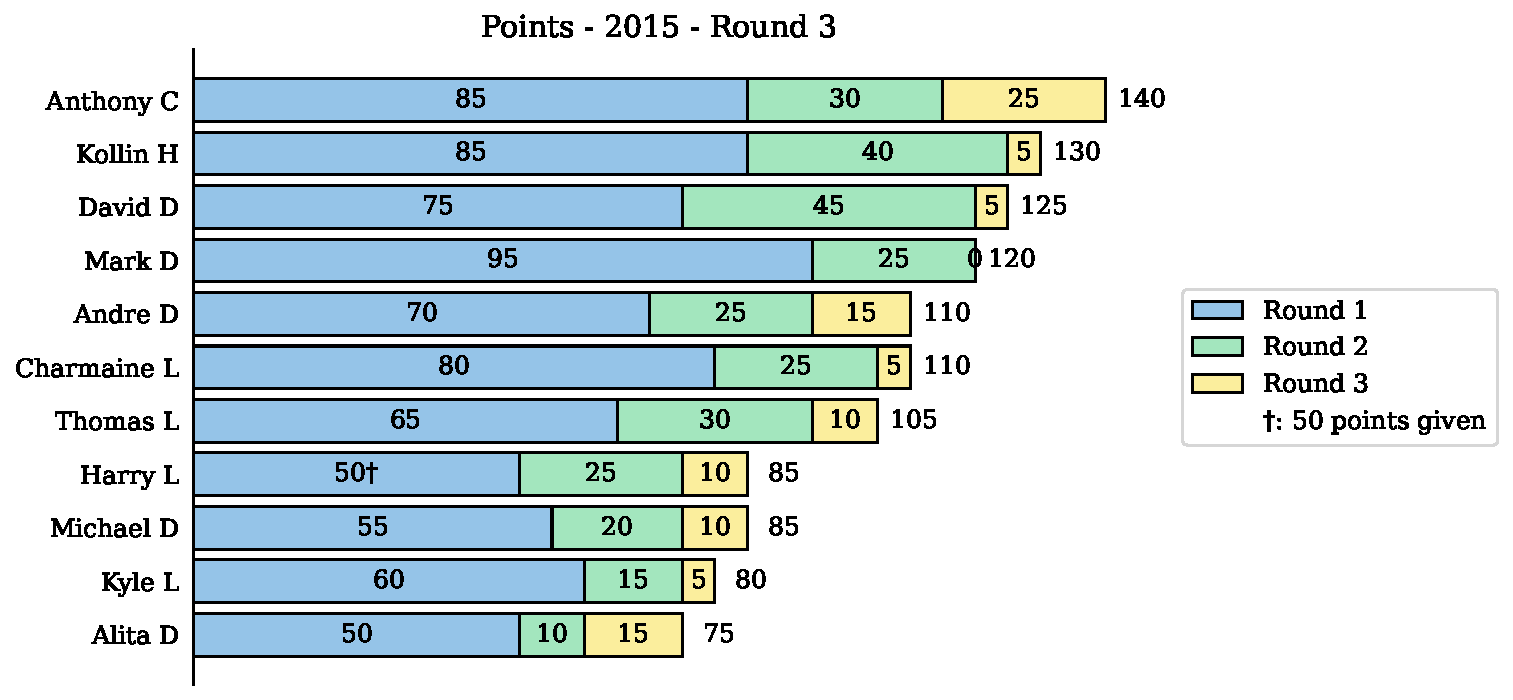
\includegraphics[width=13cm]{../../figures/2015/Points-2015-Round3.pdf}
    \end{figure}
\end{minipage}

\end{document}